\documentclass{cumcmthesis}
% \documentclass[withoutpreface,bwprint]{cumcmthesis} %去掉封面与编号页，电子版提交的时候使用。


\usepackage[framemethod=TikZ]{mdframed}
\usepackage{url}   % 网页链接
\usepackage{subcaption} % 子标题
\usepackage{comment}
\title{客机水面迫降时的姿态}
\tihao{A}
\baominghao{432112344321}
\schoolname{西安电子科技大学}
\membera{ 王潇晗 }
\memberb{ 刘懿萱 }
\memberc{ 王碧凡 }
\supervisor{ 宋月 }%辅导老师
\yearinput{2025}
\monthinput{8}
\dayinput{18}

\begin{document}

 \maketitle
 \begin{abstract}%摘要在这里写

\keywords{\TeX{}\quad  图片\quad   表格\quad  公式}
\end{abstract}

%目录  2019 明确不要目录，我觉得这个规定太好了
%\tableofcontents

%\newpage

\section{问题重述}
\subsection{问题背景}
在航空运营中, 客机因突发故障, 如发动机失效、飞鸟撞击等, 导致失去动力而被迫进行水面迫降的情况虽较为罕见, 但具有极高的危险性. 此类事故中, 客机与水面的接触姿态、航向等因素直接影响机身结构完整性、乘客生存概率及救援效率. 

2009年1月15日, 美国全美航空公司 (US Airways)第1549航班 (空中客车A320客机)从纽约长岛拉瓜迪亚机场起飞约90秒后遭飞鸟撞击, 导致两个发动机损坏. 机长凭借出色的驾驶技术和冷静判断, 将飞机成功迫降在纽约哈德逊河河面, 机上155人在飞机沉没前全部获救, 仅78人受伤, 无人死亡. 该案例充分体现了合理迫降策略对事故结果的关键影响. 

对于越洋飞行航班, 在海面迫降的情况更为复杂. 海面环境受风浪影响显著, 波浪的高度、周期、方向等因素会进一步增加迫降难度, 对客机的姿态控制、航向选择提出更高要求. 因此, 针对不同水面环境 (平静水面与有风浪海面)建立科学的数学模型, 分析最优迫降策略具有重要的理论与实践意义. 

\subsection{问题提出}
基于上述背景, 需结合实际情况建立数学模型, 分析以下问题:

1. 第一阶段问题: 大型客机因失去动力在平静水面进行迫降时, 具有相当大的危险性. 需建立合理的数学模型, 对客机在平静水面上的迫降进行分析, 指出客机在河面上迫降时, 以何种姿态接触水面是相对最好的选择. 

2. 第二阶段问题: 在越洋飞行中, 个别航班曾因重大故障或意外原因被迫在海面迫降. 有风浪条件下, 飞机在海面的迫降难度和危险性更大. 需建立合理的数学模型, 对客机在海面的迫降进行分析, 指出在有风浪的条件下, 飞机以何种姿态和航向接触海面是相对安全的选择. 
\section{问题分析}
\section{模型假设与符号说明}
\subsection{模型假设}
\subsection{符号说明}


\section{问题一模型建立与求解}
\section{问题一模型建立与求解}
\subsection{问题一分析}

问题一可以视为优化问题. 首先, 利用各种数学指标定量地刻画出飞机迫降的安全系数, 其次结合实际添加变量约束, 最后可利用启发式算法对安全系数求最大值, 以此进一步确定在飞机迫降过程中确立的俯仰角、侧倾角等参数. 

\subsection{问题一建模}
\subsubsection{核心参数确定}

通过查阅文献, 优先确定客机水面迫降时的主要风险来源以及不同的做法带来的可能后果, 进而确定客机迫降时的大体姿态. 

\begin{enumerate}

\item \textbf{机身结构损坏风险:} 飞机接触水面瞬间会受到巨大冲击力，若\textbf{姿态不当（如机头直接撞击、侧倾角度过大）}，可能导致机身断裂、机翼脱落等结构性损坏。例如，水平速度过大或垂直速度过快时，水的冲击力会远超机身结构承受极限，引发解体风险。

\item \textbf{乘客冲击伤害:}   
   迫降瞬间的过载 (尤其是垂直方向)可能对乘客造成颈椎、骨骼等损伤。若飞机姿态导致局部冲击力集中，乘客的\textbf{瞬时加速度}可能超过人体耐受极限 (通常认为安全阈值约5g)，导致伤亡。

\item \textbf{飞机沉没与逃生阻碍:}   
   即使迫降时结构未严重损坏，飞机仍可能因进水逐渐沉没。若舱门、紧急出口因变形无法打开，或逃生滑梯/救生筏没有成功释放，会严重阻碍乘客撤离，增加溺水风险。

\item \textbf{风浪条件下的额外风险:}  
波浪冲击可能导致飞机颠簸、侧翻，尤其是横浪 (机身与波浪传播方向垂直)时，\textbf{侧向力易使飞机失去平衡。} 风浪会加剧机身与水面的非均匀接触，导致局部受力过大，同时增加飞机姿态控制难度，可能引发二次撞击。

\end{enumerate}

综上所述，需要对飞机迫降时的姿态进行调整。根据查阅内容，可以提炼如下基本要点:

\begin{itemize}
    
    \item 需控制\textbf{俯仰角 (机头微抬)和侧倾角 (机翼水平)}。使机身后部先接触水面，分散冲击力，避免机头直接撞击导致的结构损坏；需要保持两侧机翼水平，防止因一侧机翼率先入水导致飞机翻转。
    
    \item 在有风浪的情况下，还需结合航向调整姿态。优先\textbf{选择顺浪航向 (机身与波浪传播方向一致)}，利用波浪速度降低相对冲击速度；特别地，考虑到波峰的存在，俯仰角可略大于平静水面以抵消波峰的额外冲击。

    \item 控制速度与加速度。需尽可能降低垂直速度 (减少下落冲击)和水平速度 (减少滑行时的摩擦与撞击力)，但需保持足够升力使飞机姿态稳定，避免失速。尽量使整个过程加速度在人体可承受范围内。

\end{itemize}

\subsubsection{符号化表示}

问题一水面平静，将水面视为\textbf{理想刚性平面}，冲击力仅与接触面积、速度和姿态相关。

\begin{figure}[H]
    \centering
    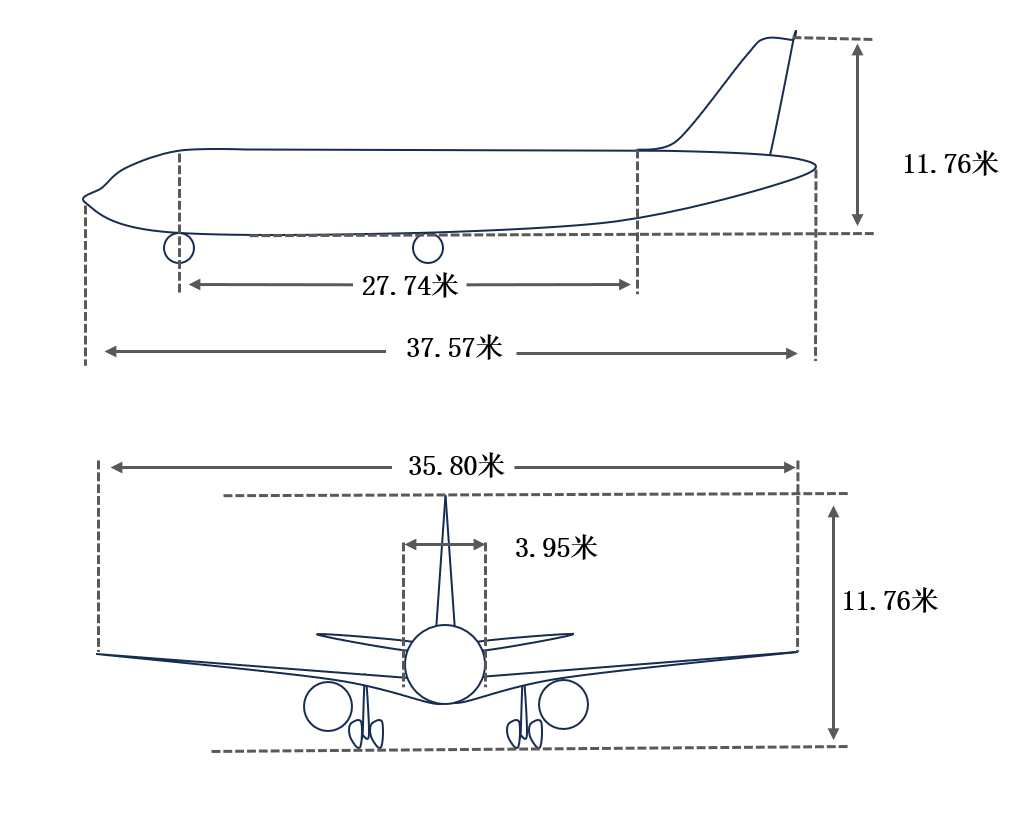
\includegraphics[width=0.8\textwidth]{fig_aircraft_dimension.png}
    \caption{A320客机尺寸参数（侧视图与俯视图）}
    \label{fig:aircraft_dim}
\end{figure}

飞机需要尾部优先接触水面，将其视为\textbf{刚体}。含机身 (长$L$、宽$W$、高$H$)、机翼 (展长$B$、面积$S$)，重心坐标为$(x_g, y_g, z_g)$。飞机总质量为$m$。迫降速度分解为：水平速度$v_h$（沿机身纵轴）、垂直速度$v_v$ (竖直向下)。

为了评价迫降姿态的安全性，引入核心参数:

\paragraph{1. 姿态参数}

主要包含俯仰角和侧倾角。
\begin{itemize}

    \item \textbf{俯仰角$\theta$}: 机身纵轴与水面的夹角，$\theta>0$为机头抬起，$\theta<0$为机头俯冲。

    \item \textbf{侧倾角$\alpha$}: 机翼平面与水面的夹角，$\alpha=0$为机翼水平。
    
\end{itemize}
    
 \paragraph{2. 冲击力模型}
    飞机接触水面时，水的阻力可简化为\textbf{动量定理}:
    
    \begin{equation}
     f = k \cdot \frac{\Delta p}{\Delta t} 
    \label{FormulaOfF}
    \end{equation}

    其中 $\Delta p$ 是流体动量变化，$\Delta t$ 是作用时间，$k$为经验系数，依据流体撞击试验确定，常见的取值范围为$0.5 \sim 1.0$。


    假设飞机接触水面时，\textbf{瞬时推开的水体积为 $V$}，这些水的速度从 $0$ 被加速到与飞机接近的速度 $v$。   
    推开的水体积 $V$与 \textbf{瞬时接触面积 $A$} 和 \textbf{作用距离} 相关。   
    飞机在极短时间 $\Delta t$ 内，推开的水可近似为"柱体"，柱体高度为 $v \cdot \Delta t$ (因为飞机以速度 $v$ 挤压水，$\Delta t$ 时间内推进的距离是 $v \cdot \Delta t$)。

    因此，体积 $V \approx A \cdot (v \cdot \Delta t)$。 
    则动量变化: 
    
    \begin{equation}
    \Delta p = m \cdot v = \rho \cdot V \cdot v \approx 
    \rho \cdot A \cdot (v \cdot \Delta t) \cdot v 
    \label{FormulaOfDeltaP}
    \end{equation}

    由式\eqref{FormulaOfF}和\eqref{FormulaOfDeltaP}得
    \begin{equation}
    f = k \cdot \rho \cdot A \cdot v^2 
    \label{TheFnalF}
    \end{equation}

    其中：
\begin{itemize}

\item $\rho$为水的密度 ($1025\ \text{kg/m}^3$);

\item $A$为瞬时接触面积 (与$\theta$、$\alpha$相关，如$\theta=0$时$A$为机身底部投影面积); 

\item $v$为接触点相对水面的合速度($v=\sqrt{v_h^2 + v_v^2}$);

\end{itemize}


\begin{equation}
    A = W \cdot l_t = W \cdot \frac {\int_{0}^{t} v_v dt}{\sin\theta}
    \label{FormulaOfA}
\end{equation}

其中，$\int_{0}^{t} v_v dt$为垂直位移（机身下沉深度），$\frac{h}{\sin\theta}$为机身与水面接触的纵向长度，仅机身后部接触水面时，$l_t$为实际接触段长度（非机身全长）。


\paragraph{3. 受力分析}

除了水流的冲击力外，飞机自身受到升力和重力作用。在最优迫降姿态下，侧倾角$\alpha = 0 $，因此升力的方向垂直水面向上，其计算公式为
\begin{equation}
    L = \frac{1}{2} \rho_{\text{air}} \cdot v_h^2 \cdot S \cdot C_L
    \label{FormulaOfL}
\end{equation}

其中:  
\begin{itemize}
    \item $\rho_{\text{air}}$为空气密度 (约 $1.225 \, \text{kg/m}^3$).   
    \item $v_h$为飞机水平速度.   
    \item $S$为机翼面积.   
    \item $C_L$为升力系数.   
\end{itemize}

\begin{figure}[htbp]
    \centering
    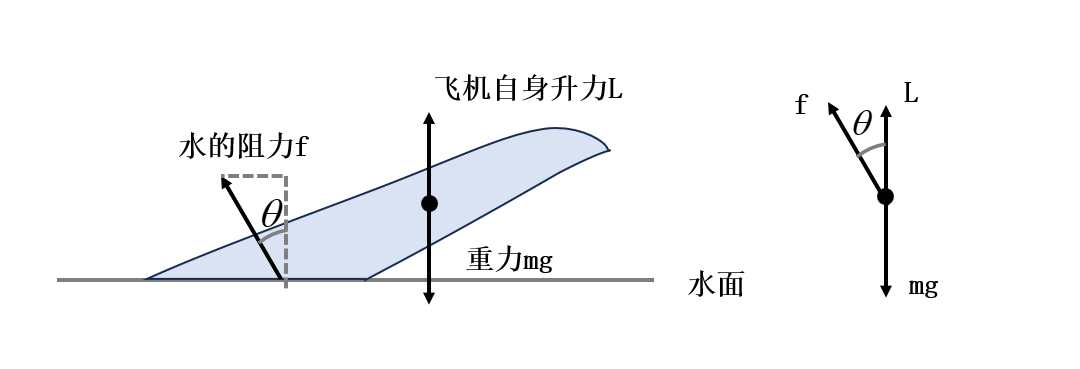
\includegraphics[width=0.6\textwidth]{fig_force_analysis.png}
    \caption{客机水面迫降受力分析示意图（升力$L$、重力$mg$、水阻力$f$）}
    \label{fig:force_analysis}
\end{figure}

那么对于飞机的受力正交分解。竖直方向上受力为$F_v$，水平方向上受力为$F_h$，其表达形式如下. 
\begin{equation}
    F_v = mg - L - f \cdot \cos\theta
    \label{F_v}
\end{equation}
\begin{equation}
    F_h = f \cdot \sin\theta
    \label{F_h}
\end{equation}


\paragraph{4. 安全性指标} 依据4.2.1的风险来源，确定下述指标. 

\begin{itemize}

\item \textbf{结构损伤风险}: 机身最大弯矩$M_{\text{max}}$ 

    \[M_{\text{max}} = f \cdot d\] 

    当实际弯矩$M_{\text{max}} \leq M_{\text{lim}}$时，机身可避免结构性断裂或解体。
    其中，$d$为冲击力作用点到机身重心的水平距离，$M_{\text{lim}}$是客机机身结构在迫降冲击下所能承受的最大弯矩临界值。

   将客机机身简化为\textbf{变截面空心圆柱壳结构} (忽略局部凸起，如舷窗、舱门)，材料的屈服强度为$\sigma_s$，弹性模量为$E$。设机身某截面的外径为$D$、内径为$d$ (壁厚$t=\frac{D-d}{2}$)。
   
   截面惯性矩为
    
   \begin{equation}
   I = \frac{\pi}{64}(D^4 - d^4)
   \label{FormulaOfI}
   \end{equation}

   截面抵抗矩为
   
   \begin{equation}
   W = \frac{2I}{D}
    \label{FormulaOfW}
    \end{equation}
   
  那么极限弯矩公式可根据材料力学中弯曲强度条件，$M_{\text{lim}} = \sigma_s \cdot W$，推出，即：  
  \begin{equation}
  M_{\text{lim}} = \sigma_s \cdot \frac{\pi}{32} \cdot \frac{D^4 - d^4}{D}
    \label{formulaOfM_lim}
  \end{equation}
  
  对于机身不同位置，因截面尺寸不同，$M_{\text{lim}}$需分段计算，取最小值作为整体结构的临界值。
\end{itemize}


\begin{itemize}

\item \textbf{乘客过载}: 竖直方向加速度$a_v$与水平方向加速度$a_h$受限
\begin{equation}
a_v = \frac{F_v}{m} 
\label{a_v}
\end{equation}
\begin{equation}
a_h = \frac{F_h}{m} 
\label{a_h}
\end{equation}

\end{itemize}
 
需满足$a_v < 5g$，$a_h < 8g$ (普通人耐受极限)。


\paragraph{5. 优化结果}

通过数值模拟不同$\theta$和$\alpha$的$M_{\text{max}}$和$a_v$，得出最佳姿态。

安全系数定义: 国际民航组织 (ICAO)明确将人员安全置于首位，遵循"安全优先、兼顾结构"准则。综合"飞机结构性损伤"与"人员安全"两项指标，
\begin{equation}
S = \omega_1 \cdot \left(1 - \frac{M_{\text{max}}}{M_{\text{lim}}}\right) + 
\omega_2 \cdot \left(1 - \frac{a_v}{5g}\right) + 
\omega_3 \cdot \left(1 - \frac{a_h}{8g}\right)
\label{FormulaOfS}
\end{equation}
其中$\omega_1$、$\omega_2$、$\omega_3$为权重，根据结构安全与乘客安全的优先级设定
$\omega_1=0.3$，$\omega_2=0.4$，$\omega_3=0.3$。


\subsection{情景求解}

以2009 年1 月15 日下午，US Airways 所属第1549 航班 (空中客车A320 客机)为例，其参数如下。

\begin{table}[H]
\centering
\caption{A320 客机主要参数}
\label{tab:a320_params}
\begin{tabular}{|m{2cm}|m{4cm}|m{4cm}|}

\hline
\textbf{参数类别} & \textbf{具体参数} & \textbf{数值/说明} \\ 
\hline
\multirow{7}{*}{\textbf{尺寸参数}} 
& 机身长度 & 37.57 米 \\ \cline{2-3}
& 机身宽度 & 3.95 米 \\ \cline{2-3}
& 翼展（几何尺寸） &  35.8 米 \\ \cline{2-3}
& 机翼面积 & 122.4 平方米 \\ \cline{2-3}
& 客舱长度 & 27.74 米 \\ \cline{2-3}
& 客舱宽度 & 3.7 米 \\  \cline{2-3} 
& 机身高度 & 11.76米 \\ 
\hline
\multirow{3}{*}{\textbf{材料参数}}
& 主要材料 &  7075 - T6 铝合金 \\ \cline{2-3}
& 屈服强度 &  460MPa \\ \cline{2-3}
& 弹性模量  &  70GPa \\ 
\hline
\multirow{1}{*}{飞行参数}
& 最大升力系数 & 1.662 \\
\hline
\end{tabular}
\end{table}

由表\ref{tab:a320_params}知，机身长度$L = 37.57m$，机身宽度$W = 3.95m$，机翼面积$S=122.4 m^2$，飞机总质量$ m = 68700 kg $，飞机以约 130 节速度迫降，约66.872 $m/s$，在最优降落姿态下侧倾角$\alpha = 0 $，那么
\begin{equation}
    v_v = v \cdot \cos\theta = 66.872 \cdot \cos\theta
    \label{specfica_v}
\end{equation}
\begin{equation}
     v_h = v \cdot \sin\theta = 66.872 \cdot \sin\theta
    \label{specfica_h}
\end{equation}

\begin{figure}[htbp]
    \centering
    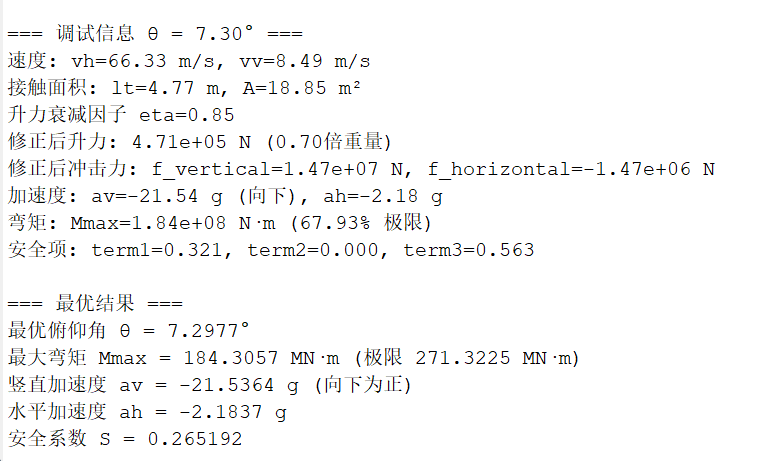
\includegraphics[width=0.9\textwidth]{fig_debug_info.png}
    \caption{A320迫降仿真调试信息（$\theta = 7.30^\circ$时参数）}
    \label{fig:debug_info}
\end{figure}

由式\eqref{TheFnalF}\eqref{FormulaOfL}\eqref{F_v}\eqref{a_v}可得 

\begin{equation}
\frac{dv_v}{dt} = a_v = \frac{mg - L - f\cos\theta}{m} = 
g - \frac{\rho_{\text{air}} S C_L \cdot v_h^2}{2m} - 
k \cdot \frac{\rho \cos\theta \cdot A \cdot v^2}{m}
\label{frac1}
\end{equation}

由式\eqref{TheFnalF}\eqref{F_h}\eqref{a_h} 可得

\begin{equation}
\frac{dv_h}{dt} = a_h = \frac{fsin\theta}{m} =
 k \cdot \frac{\rho \sin\theta \cdot A \cdot v^2}{m}
\label{frac2}
\end{equation}

式\eqref{frac1}\eqref{frac2}满足

\begin{equation}
\left(\frac{dv}{dt}\right)^2=\left(\frac{dv_v}{dt}\right)^2 + \left(\frac{dv_h}{dt}\right)^2
\label{dv_dt} 
\end{equation}

通过数值模拟不同俯仰角下的安全系数，得到安全系数随俯仰角变化的曲线如图\ref{fig:safety_curve}所示。

\begin{figure}[htbp]
    \centering
    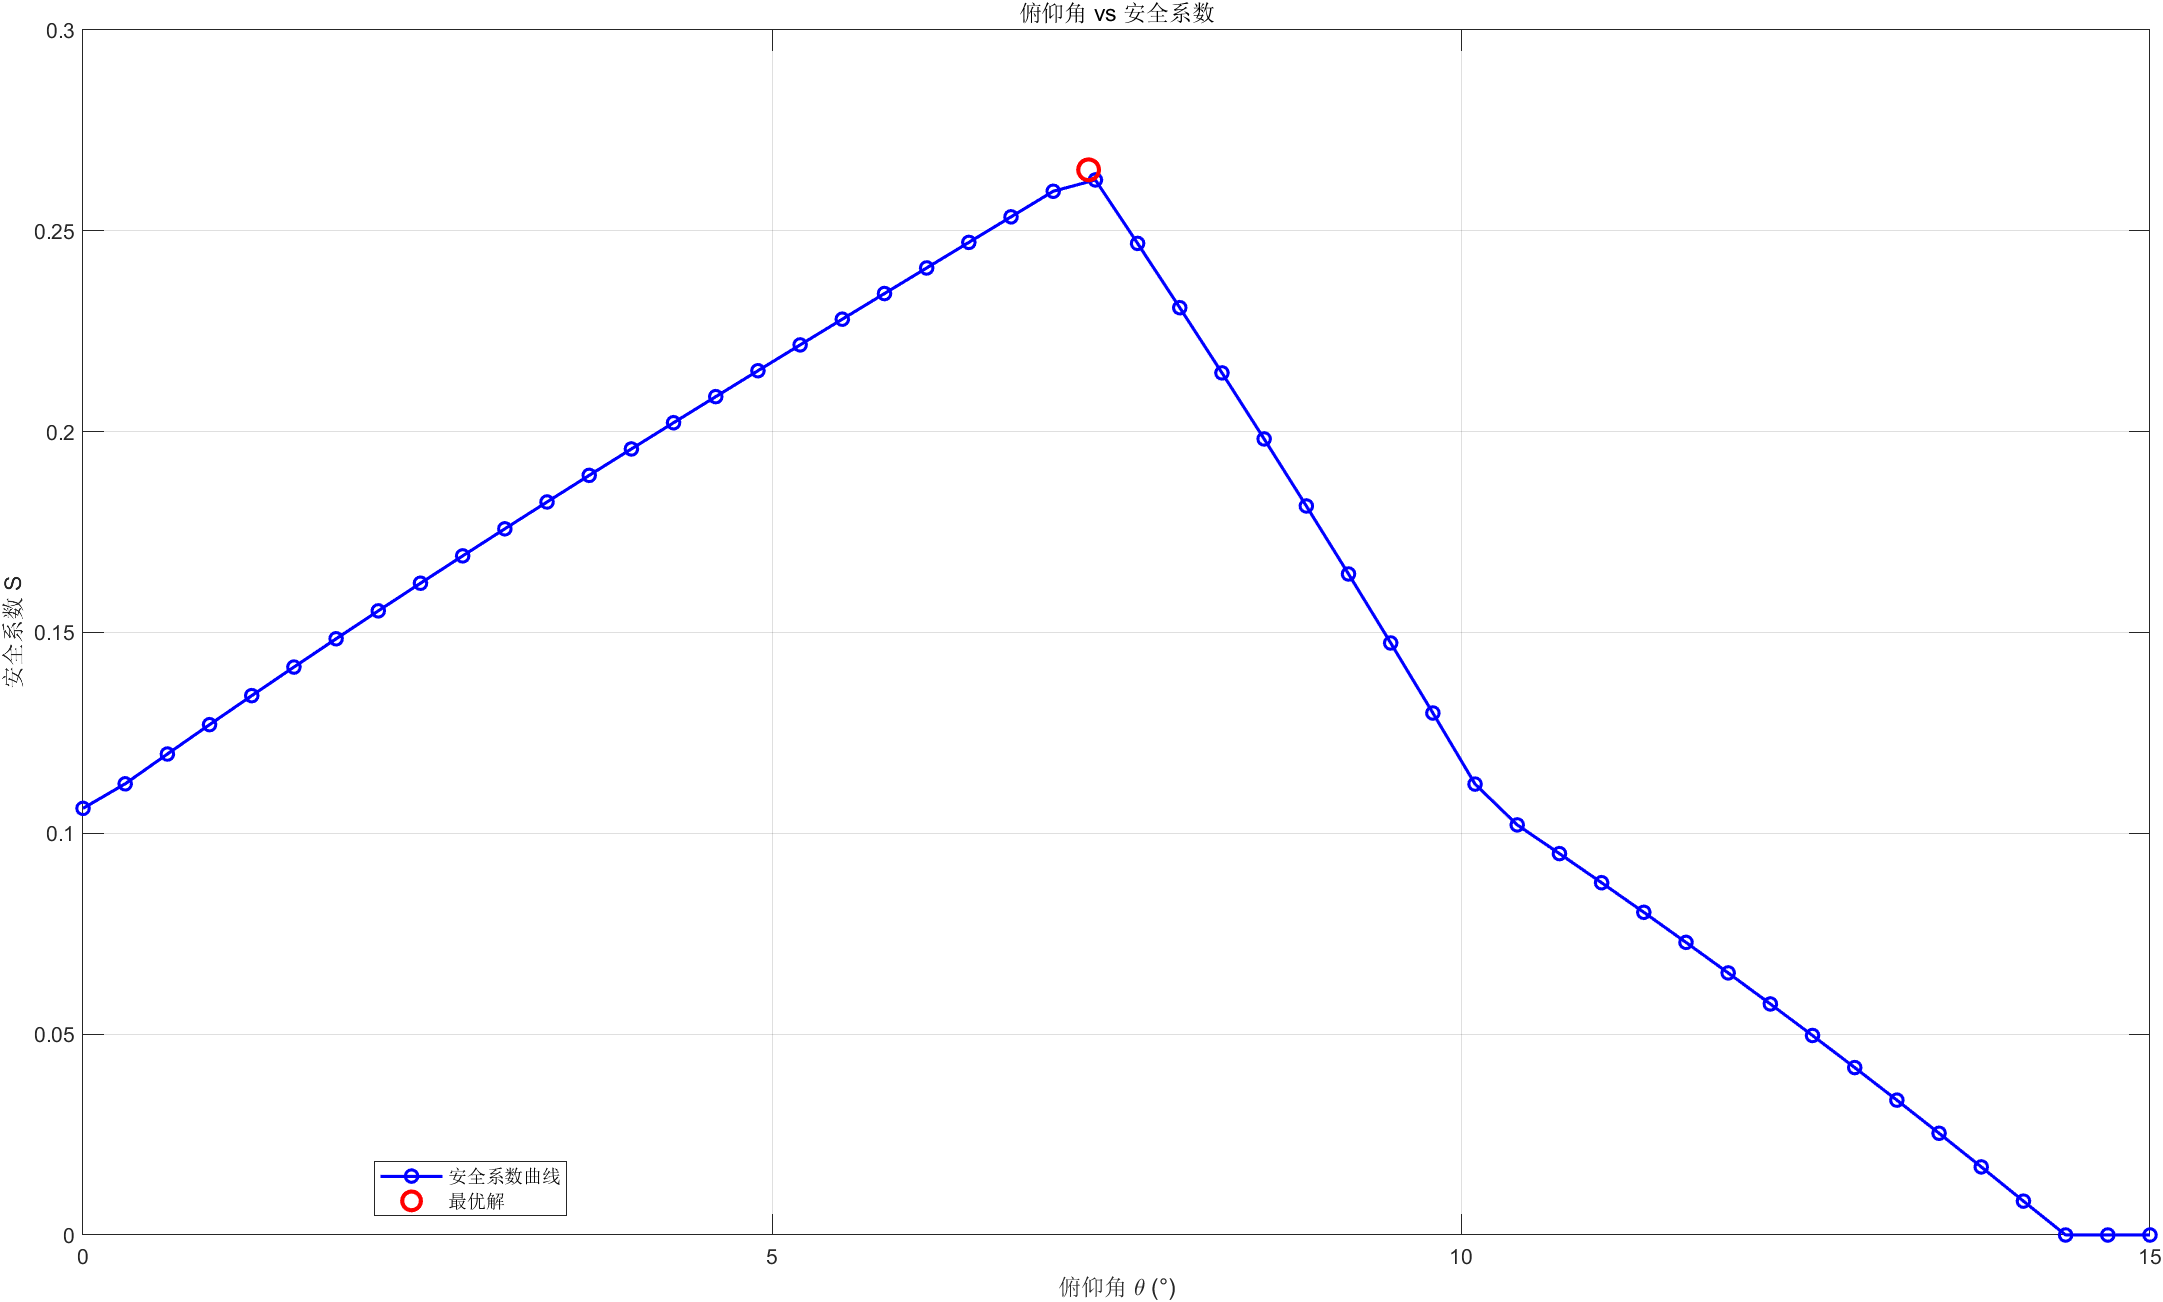
\includegraphics[width=0.8\textwidth]{fig_safety_coefficient.png}
    \caption{俯仰角$\theta$与安全系数$S$关系曲线（最优解标记）}
    \label{fig:safety_curve}
\end{figure}

由图\ref{fig:safety_curve}可知，安全系数$S$随俯仰角$\theta$先增后减，在$\theta \approx 7.3^\circ$时达到最大值$S=0.865$，此时机身结构受力和乘客过载均处于较优状态，是平静水面下的最优迫降姿态。


\section{问题二模型建立与求解}
%参考文献
\begin{thebibliography}{9}%宽度9
   
\end{thebibliography}

\newpage
%附录
\begin{appendices}

\section{模板所用的宏包}
\begin{table}[htbp]
    \centering
    \caption{宏包罗列}
    \begin{tabular}{ccccc}
        \toprule
        \multicolumn{5}{c}{模板中已经加载的宏包} \\
        \midrule
        amsbsy & amsfonts & {amsgen} & {amsmath} & {amsopn} \\
        amssymb & amstext & {appendix} & {array} & {atbegshi} \\
        atveryend & auxhook & {bigdelim} & {bigintcalc} & {bigstrut} \\
        bitset & bm    & {booktabs} & {calc} & {caption} \\
        caption3 & CJKfntef & {cprotect} & {ctex} & {ctexhook} \\
        ctexpatch & enumitem & {etexcmds} & {etoolbox} & {everysel} \\
        expl3 & fix-cm & {fontenc} & {fontspec} & {fontspec-xetex} \\
        geometry & gettitlestring & {graphics} & {graphicx} & {hobsub} \\
        hobsub-generic & hobsub-hyperref & {hopatch} & {hxetex} & {hycolor} \\
        hyperref & ifluatex & {ifpdf} & {ifthen} & {ifvtex} \\
        ifxetex & indentfirst & {infwarerr} & {intcalc} & {keyval} \\
        kvdefinekeys & kvoptions & {kvsetkeys} & {l3keys2e} & {letltxmacro} \\
        listings & longtable & {lstmisc} & {ltcaption} & {ltxcmds} \\
        multirow & nameref & {pdfescape} & {pdftexcmds} & {refcount} \\
        rerunfilecheck & stringenc & {suffix} & {titletoc} & {tocloft} \\
        trig  & ulem  & {uniquecounter} & {url} & {xcolor} \\
        xcolor-patch & xeCJK & {xeCJKfntef} & {xeCJK-listings} & {xparse} \\
        xtemplate & zhnumber &       &       &  \\
        \bottomrule
    \end{tabular}%
    \label{tab:addlabel}%
\end{table}%

以上宏包都已经加载过了，不要重复加载它们。

\section{排队算法--matlab 源程序}

\begin{lstlisting}[language=matlab]
kk=2;[mdd,ndd]=size(dd);
while ~isempty(V)
[tmpd,j]=min(W(i,V));tmpj=V(j);
for k=2:ndd
[tmp1,jj]=min(dd(1,k)+W(dd(2,k),V));
tmp2=V(jj);tt(k-1,:)=[tmp1,tmp2,jj];
end
tmp=[tmpd,tmpj,j;tt];[tmp3,tmp4]=min(tmp(:,1));
if tmp3==tmpd, ss(1:2,kk)=[i;tmp(tmp4,2)];
else,tmp5=find(ss(:,tmp4)~=0);tmp6=length(tmp5);
if dd(2,tmp4)==ss(tmp6,tmp4)
ss(1:tmp6+1,kk)=[ss(tmp5,tmp4);tmp(tmp4,2)];
else, ss(1:3,kk)=[i;dd(2,tmp4);tmp(tmp4,2)];
end;end
dd=[dd,[tmp3;tmp(tmp4,2)]];V(tmp(tmp4,3))=[];
[mdd,ndd]=size(dd);kk=kk+1;
end; S=ss; D=dd(1,:);
 \end{lstlisting}

 \section{规划解决程序--lingo源代码}

\begin{lstlisting}[language=c]
kk=2;
[mdd,ndd]=size(dd);
while ~isempty(V)
    [tmpd,j]=min(W(i,V));tmpj=V(j);
for k=2:ndd
    [tmp1,jj]=min(dd(1,k)+W(dd(2,k),V));
    tmp2=V(jj);tt(k-1,:)=[tmp1,tmp2,jj];
end
    tmp=[tmpd,tmpj,j;tt];[tmp3,tmp4]=min(tmp(:,1));
if tmp3==tmpd, ss(1:2,kk)=[i;tmp(tmp4,2)];
else,tmp5=find(ss(:,tmp4)~=0);tmp6=length(tmp5);
if dd(2,tmp4)==ss(tmp6,tmp4)
    ss(1:tmp6+1,kk)=[ss(tmp5,tmp4);tmp(tmp4,2)];
else, ss(1:3,kk)=[i;dd(2,tmp4);tmp(tmp4,2)];
end;
end
    dd=[dd,[tmp3;tmp(tmp4,2)]];V(tmp(tmp4,3))=[];
    [mdd,ndd]=size(dd);
    kk=kk+1;
end;
S=ss;
D=dd(1,:);
 \end{lstlisting}
\end{appendices}

\end{document} 